\section{V-Shape Formation Design} \label{sec:0design}
The V-shape formation is chosen due to its advantages in improving maneuverability and enhancing visibility for UAVs. Its modeling and design principles are presented as follows. 
\subsection{UAV model}
\begin{figure}
    \centering
    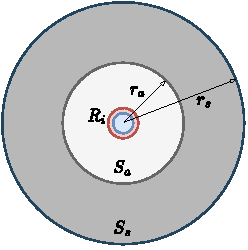
\includegraphics[width=0.3\textwidth]{paper1/images/model.pdf}
    \caption{The sensing range $r_s$ and alert range $r_a$ ($r_a<r_s$) of a UAV $R_i$}
    \label{fig:chap2_model}
\end{figure}
 
The formation consists of $n$ identical UAVs, each equipped with sensory modules for positioning and navigation such as Lidar, GPS and inertial measurement unit (IMU). The UAV is also equipped with a communication module that allows peer-to-peer communication among the UAVs. At height $h$, a UAV $R_i$ is modeled as a particle moving in a 2D plane located at that height with position $p_i$ and heading angle $\psi_i$. The single-integrator kinematic model of UAV $R_i$ can be expressed as follows:
\begin{equation}
    \dot{p}_i = u_i,
\end{equation}
where $u_i=[u_{ix},u_{iy}]^T$ is the velocity vector of UAV $R_i$. The heading angle $\psi_i$ then can be obtained as:
\begin{equation}
    \psi_i=\text{atan2}(u_{iy},u_{ix}).
\end{equation}

The communication range of each UAV $R_i$ is divided into two areas including the sensing area $S_s$ with radius $r_s$ and the alert area $S_a$ with radius $r_a<r_s$ so that $S_a\subset S_s$, as illustrated in Figure \ref{fig:chap2_model}.

\subsection{V-shape formation}
\begin{figure}
    \centering
    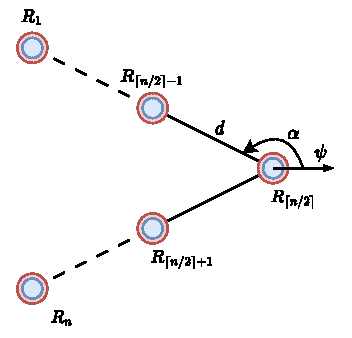
\includegraphics[width=0.4\textwidth]{paper1/images/v-shape.pdf}
    \caption{Illustration of the V-shape formation}
    \label{fig:chap2_vshape}
\end{figure}
In this work, the V-shape formation is constructed by two wings \cite{Dang2019}, as shown in Figure \ref{fig:chap2_vshape}. The wings are described by the desired distances between consecutive UAVs, $d$, and the bearing angle between the formation heading and each wing, $\alpha$. Without loss of generality, choose UAV $R_l$, with $l=\left\lceil{n}/{2}\right\rceil$, as the leader UAV located at the forefront of the formation. The desired distance $d_i$ and angle $\alpha_i$ between UAV $R_i$, $i\neq l$, and UAV $R_l$ are determined as follows:
\begin{equation}
\begin{aligned}
    d_i&=d\left\vert l-i\right\vert,\\
    \alpha_{i}&=\left\{ \begin{array}{cc}
\psi_{l}+\alpha & \text{if }i<l\\
\psi_{l}-\alpha & \text{if }i>l
\end{array}\right.
\end{aligned}
\label{eqn:chap2_desired}
\end{equation}

Thus, the desired position of UAV $R_i$ can be obtained as follows:
\begin{equation}
    p_i^d=p_l+d_i\left[\begin{array}{c}
\cos\alpha_{i}\\
\sin\alpha_{i}
\end{array}\right].
\label{eqn:chap2_desired_pose}
\end{equation}